% oil_mc_pres.tex

\documentclass{beamer}
\usepackage{url} 
\usepackage{amsmath}
\usepackage{esdiff} %for writing partial derivatives

\usetheme{default}

\title[oil]{Estimating the Effect of Price on Oil Production: Evidence from the Norwegian Continental Shelf}
\author[Mauritzen]{Johannes Mauritzen \\ NHH Norwegian School of Economics \\
jmaurit@gmail.com \\
\url{jmaurit.github.io\\#oil\_prices}}
\institute[NHH]{
 % Department of Business and Management Science\\
 % NHH Norwegian School of Economics\\[1ex]
  % \texttt{johannes.mauritzen@nhh.no}
}
\date{\today}

\begin{document}

%--- the titlepage frame -------------------------%
\begin{frame}[plain]
  \titlepage
\end{frame}

\begin{frame}
	\begin{figure}
	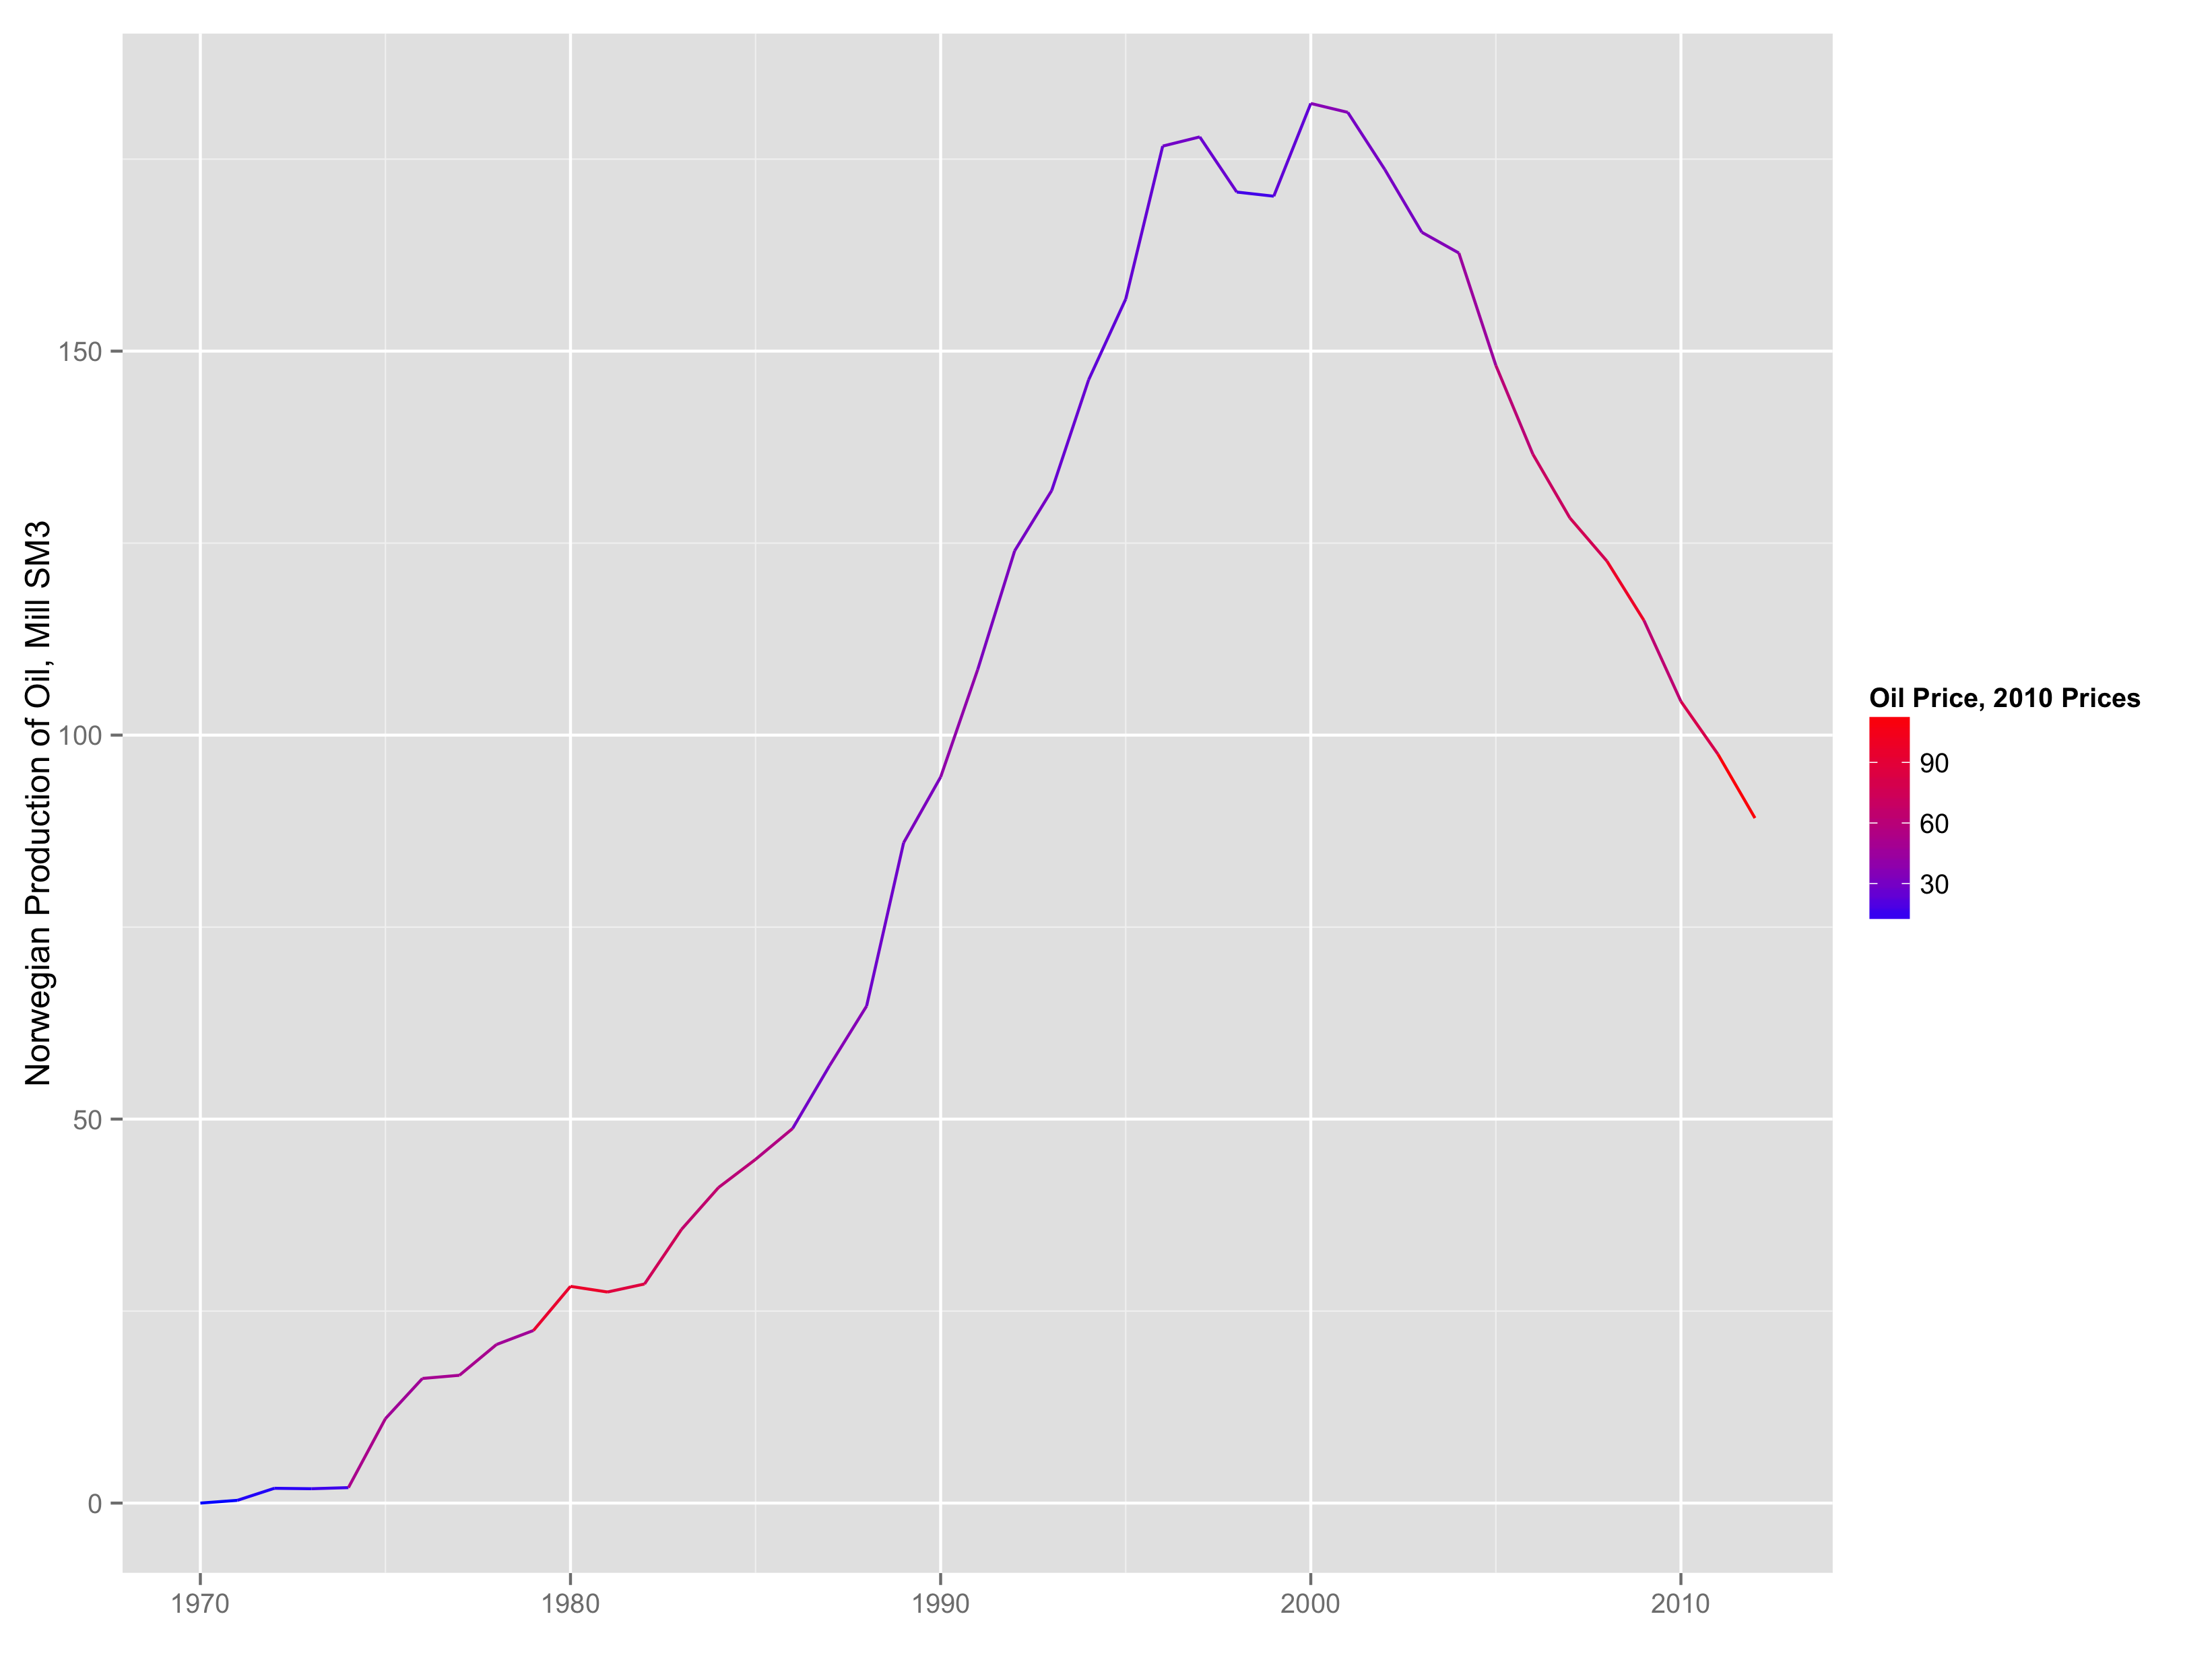
\includegraphics[width=1\textwidth]{figures/oil_decline.png}
	% \caption{The top panel shows the production from the largest 10 oil fields, whose starting times are temporally correlated with each other.  The total production over time is bell-shaped, as shown by the bottom panel.}
	\label{oil_decline}
\end{figure}
\end{frame}

\begin{frame}[plain]
	Main Results
	\begin{itemize}
		\item No significant contemporary effect of oil price on field production (within 3 years)
		\item Slight lagged effect found after 4-8 years, magnitude of around 2\%
		\item Most of this effect seems to come in the Planning stage of an oil field
		\item Little to no effect - contemporary or lagged - in depleting fields
	\end{itemize}
\end{frame}

\begin{frame}
	\begin{figure}
		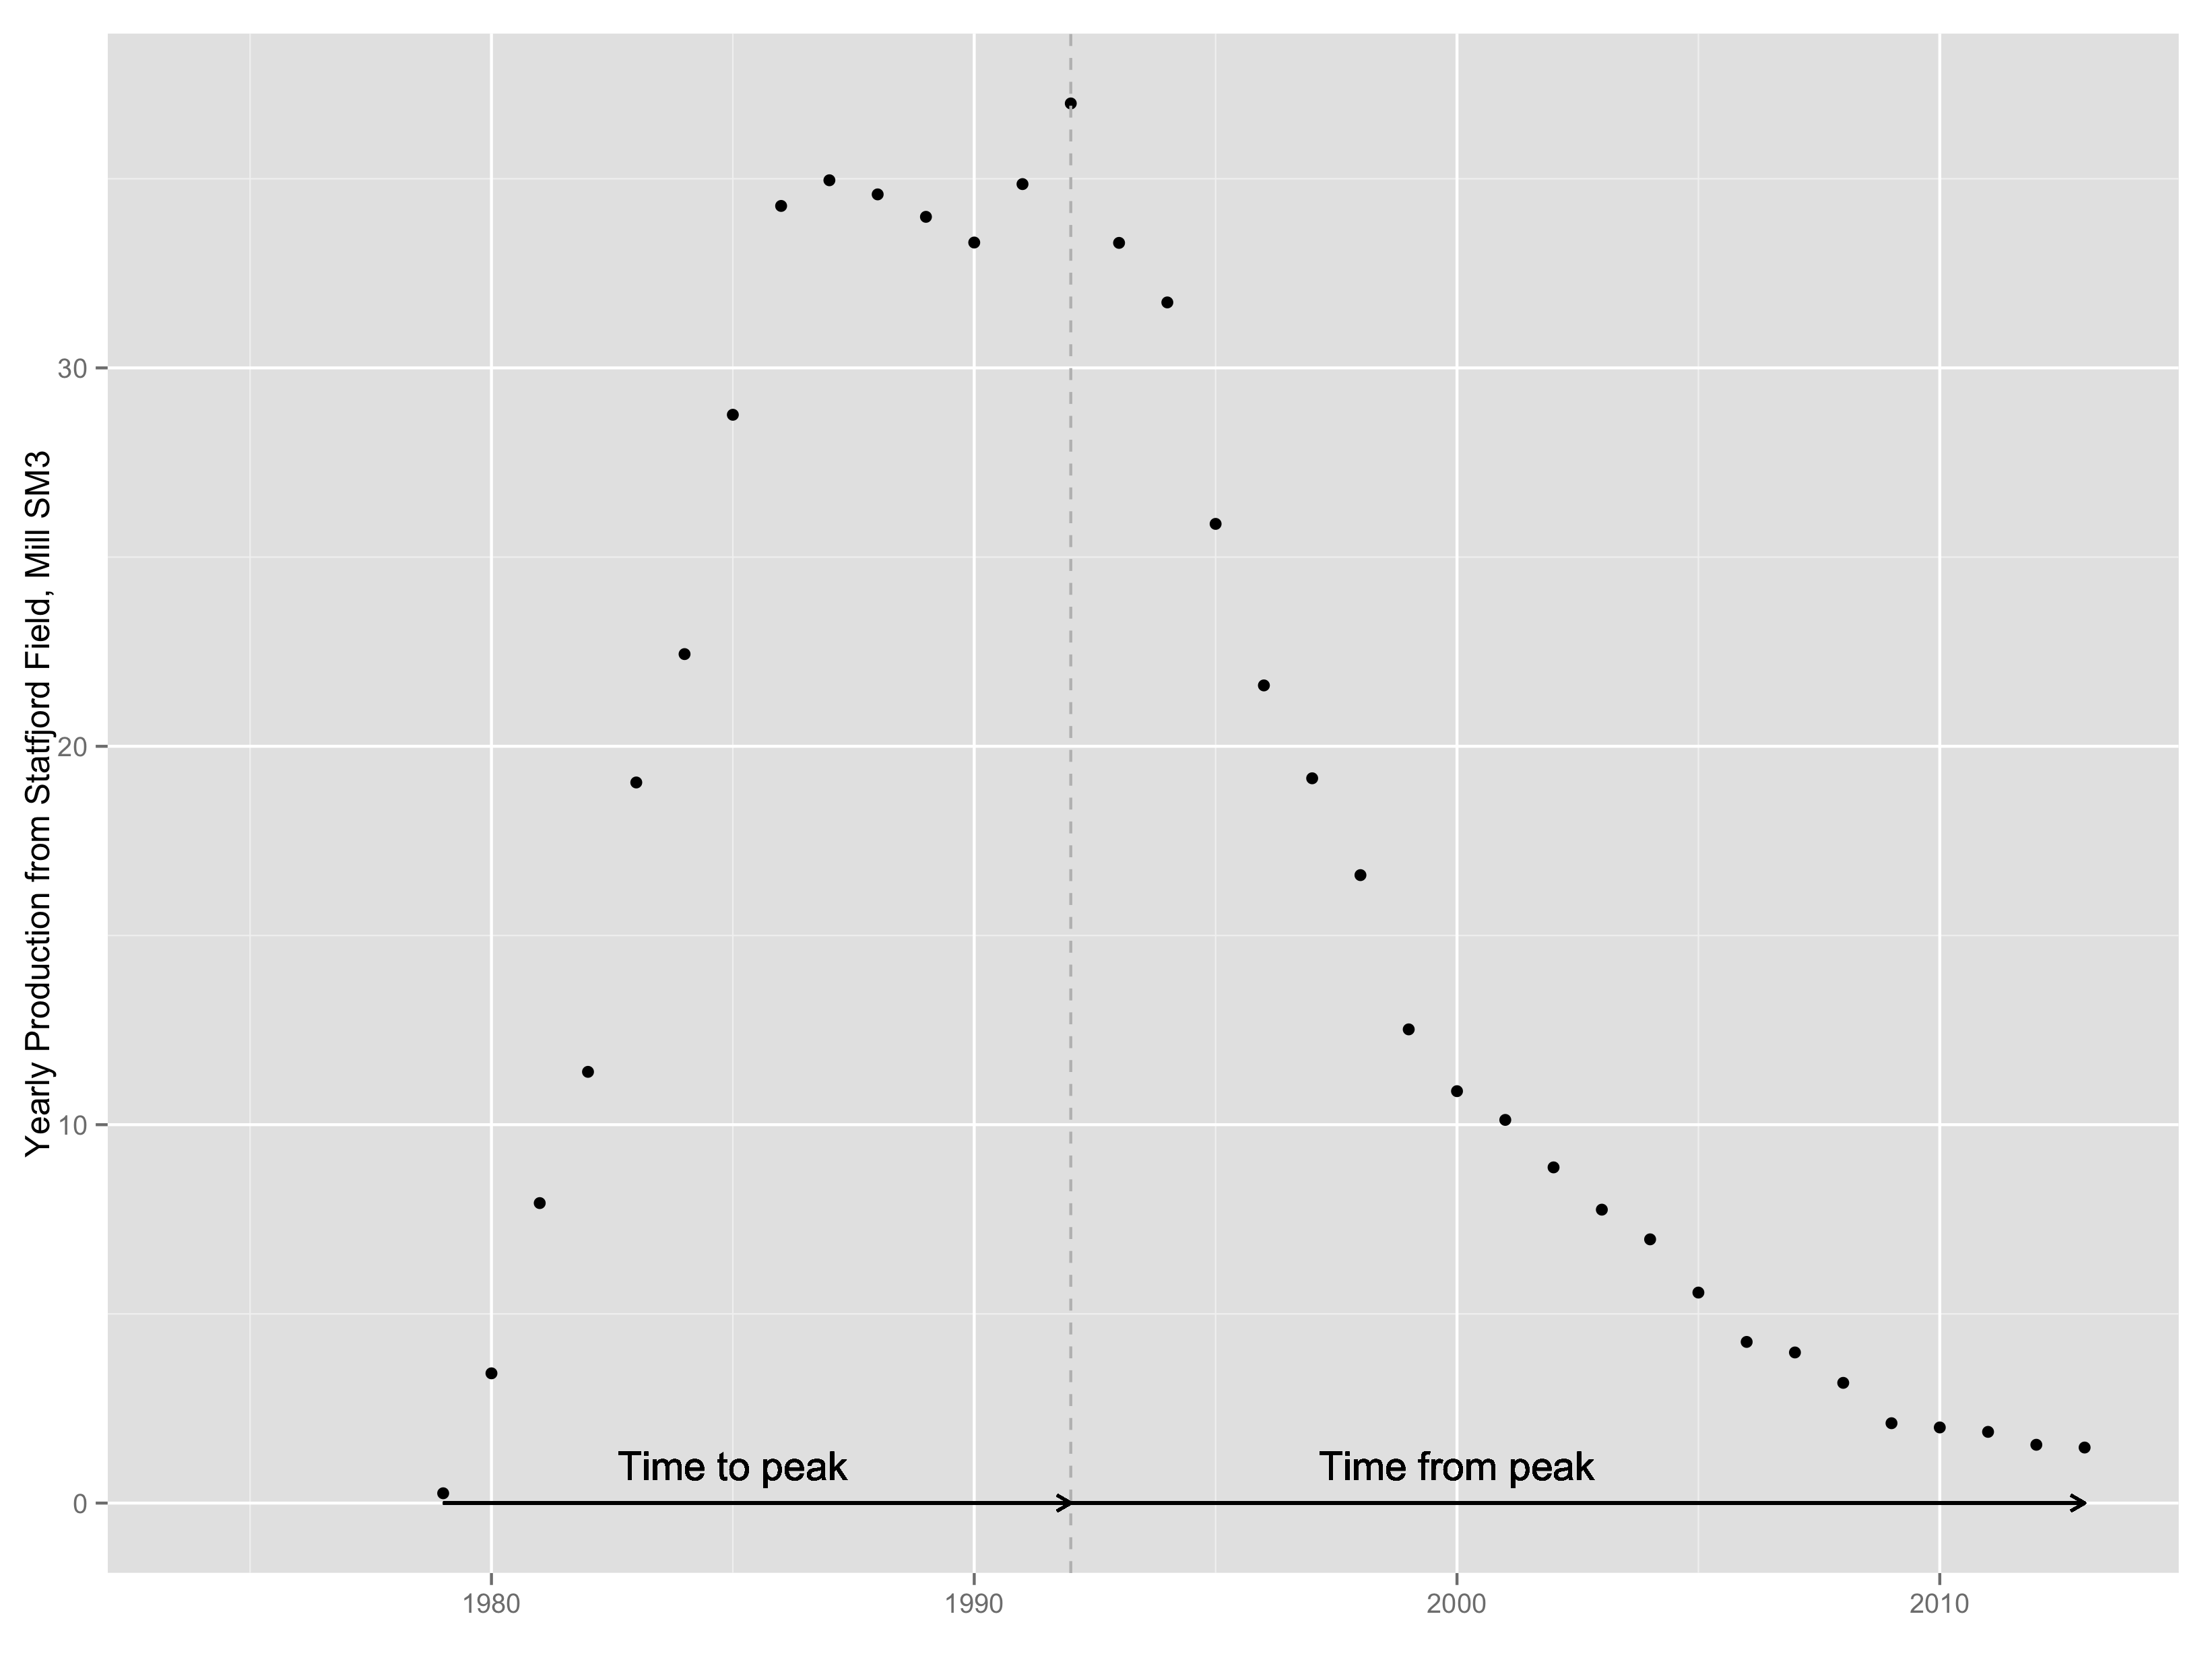
\includegraphics[width=1\textwidth]{figures/statfjord_dem_print.png}
		\label{statfjord_dem}
	\end{figure}
\end{frame}

\begin{frame}[plain]
	\begin{equation}
		\begin{split}
		 Log(Production_{i,t}) & = \alpha_0 + \alpha_1 time\_to\_peak_{i,t} + \alpha_2 time\_to\_peak_{i,t}^2 \\
		& \quad + \alpha_3 time\_to\_peak_{i,t}^3  + \alpha_4 peak\_to\_end_{i,t} \\
		& \quad + \alpha_5 peak\_to\_end_{i,t}^2 \\
		& \quad + \alpha_6 peak\_to\_end_{i,t}^3 + \gamma total\_recoverable\_oil_i \\
		& \quad + \beta_1 oil\_price + \beta_2 oil\_price\_l1 + ...+ \epsilon
		\end{split}
	\label{glm_eqn}
		\end{equation}
\end{frame}

\begin{frame}[plain]
	\begin{figure}
		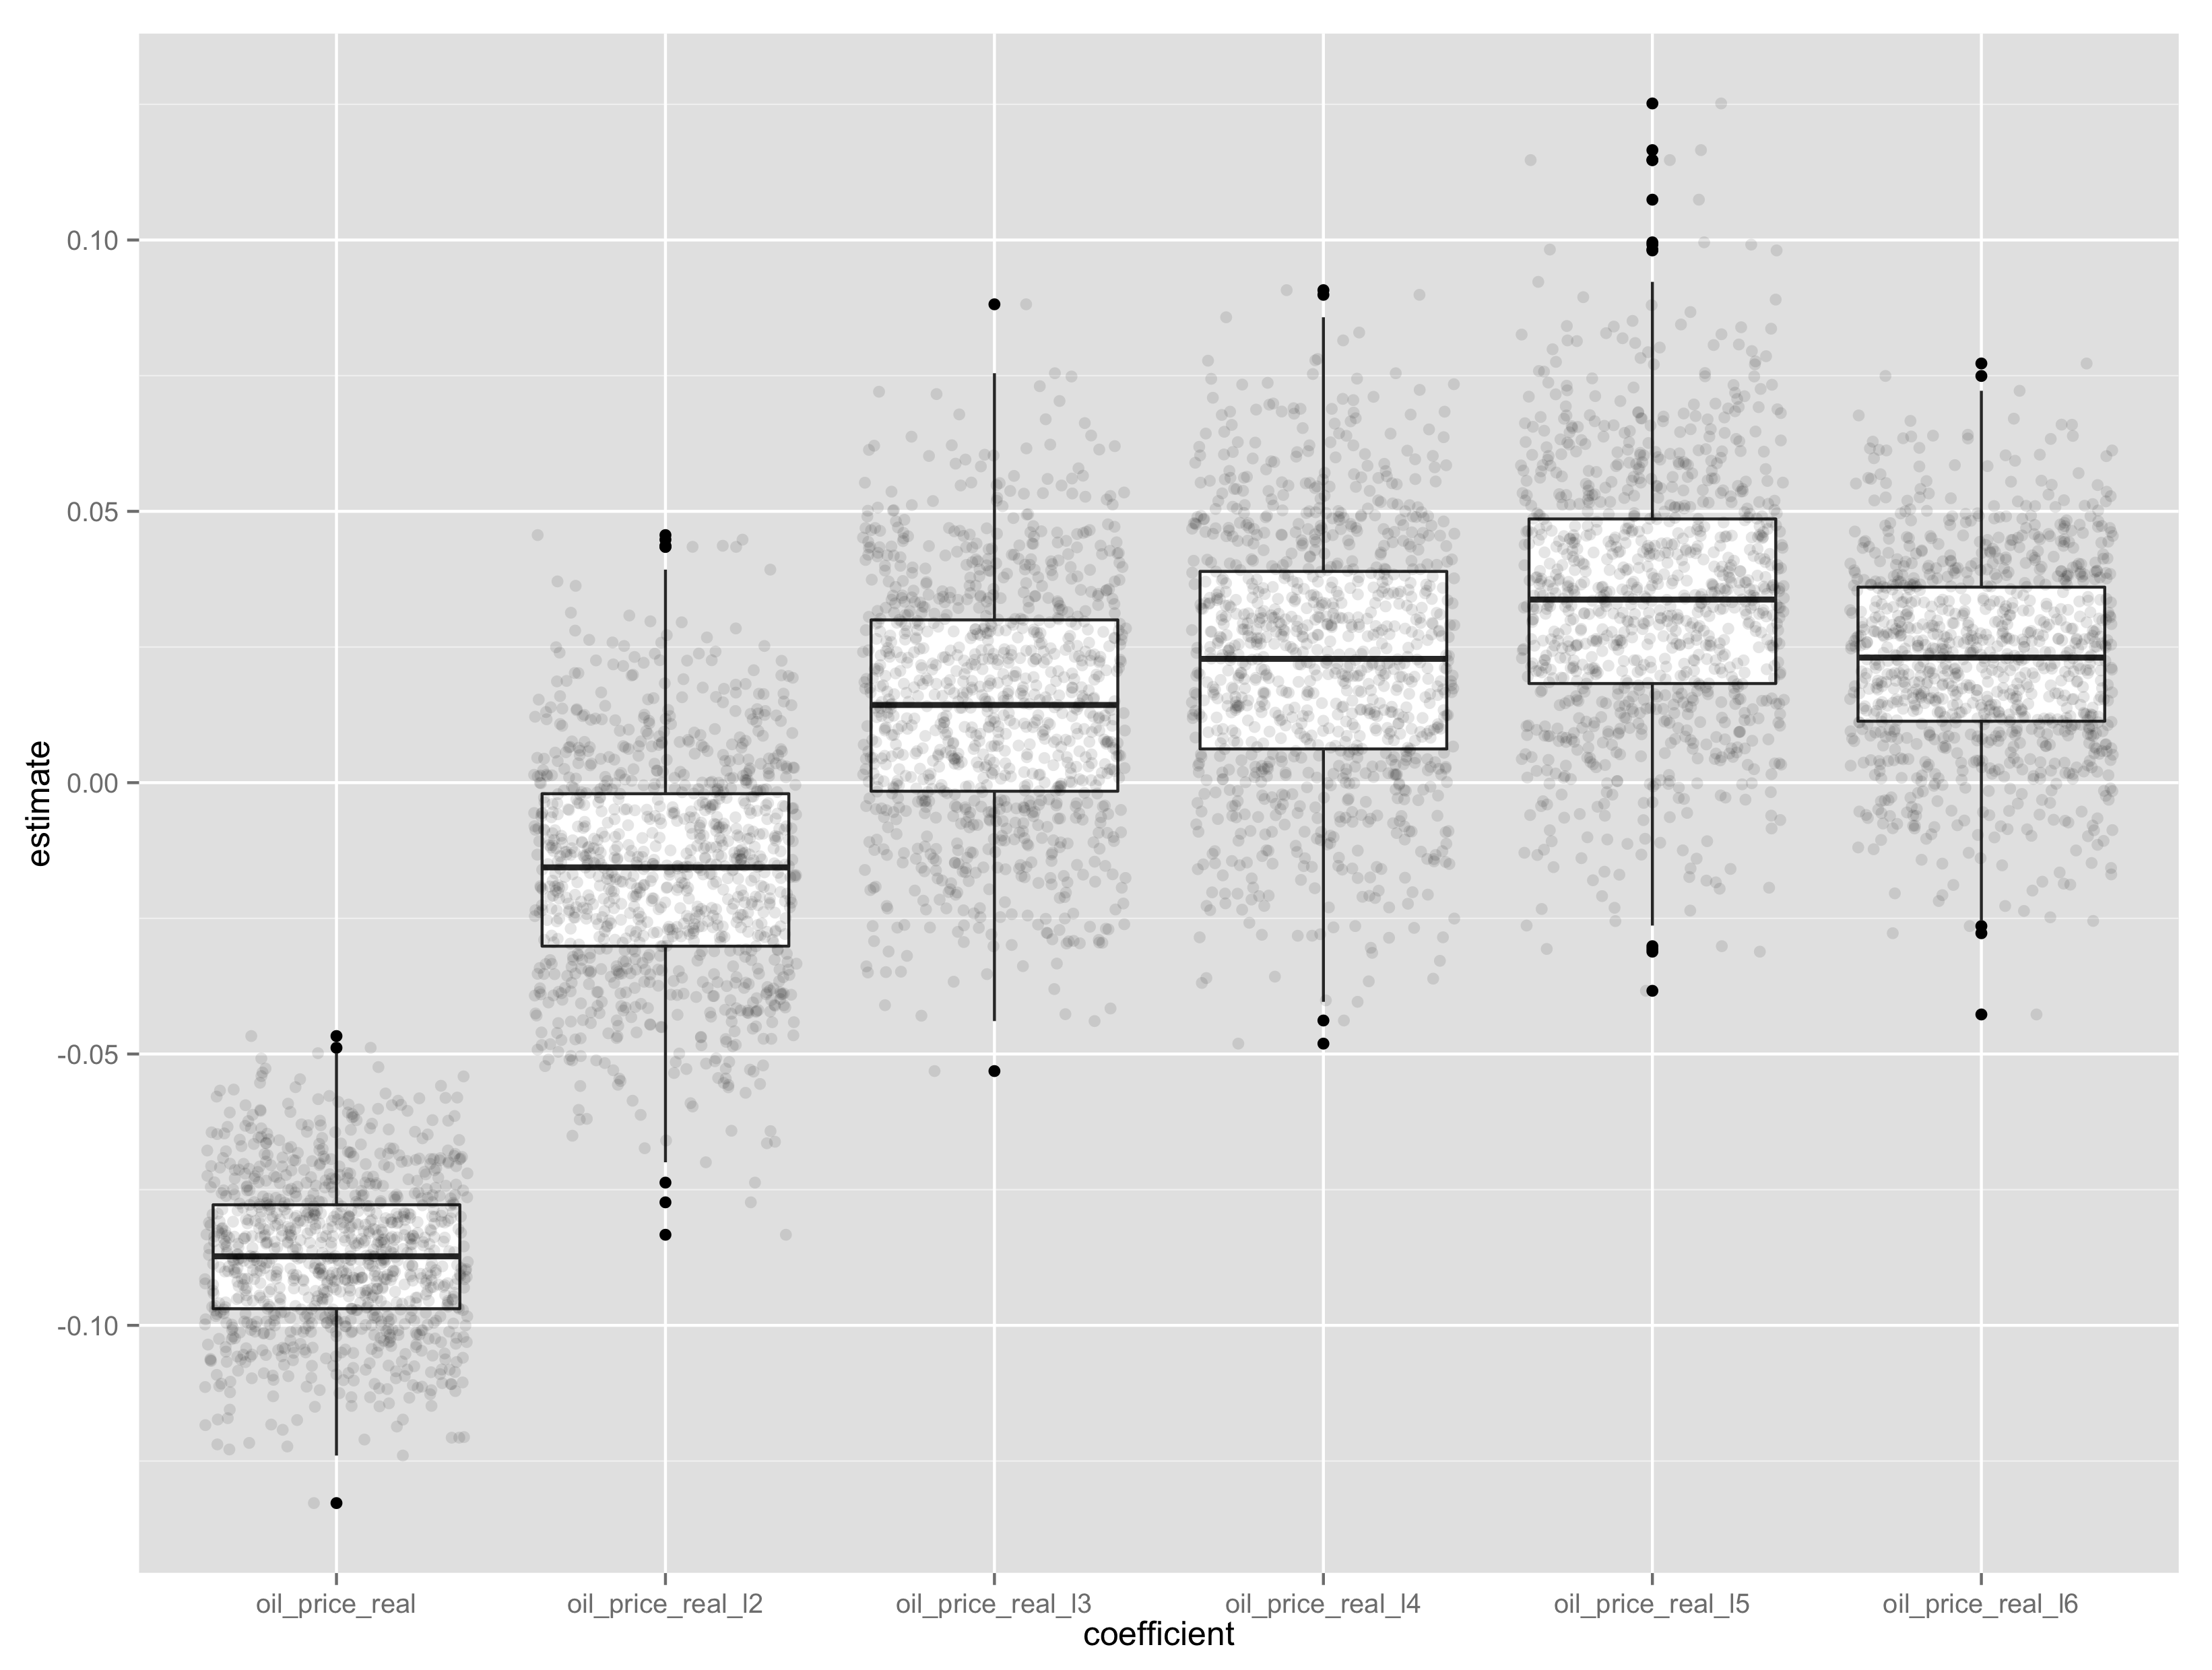
\includegraphics[width=.8\textwidth]{figures/glm_dirty_box.png}
		\label{glm_dirty_box}
	\end{figure}
\end{frame}


\begin{frame}[plain]
	\begin{equation}
	\begin{split}
		Log(Production_{i,t})&=f(time\_to\_peak_{i,t}, total\_recoverable\_oil_i) \\
		& \quad + f(peak\_to\_end_{i,t}, total\_recoverable\_oil_i) \\
		& \quad + \beta_1 oil\_price + \beta_2 oil\_price\_l1 + ... +  \epsilon
	\end{split}
	\label{gam_price_eqn}
	\end{equation}
\end{frame}

\begin{frame}
\begin{figure}
	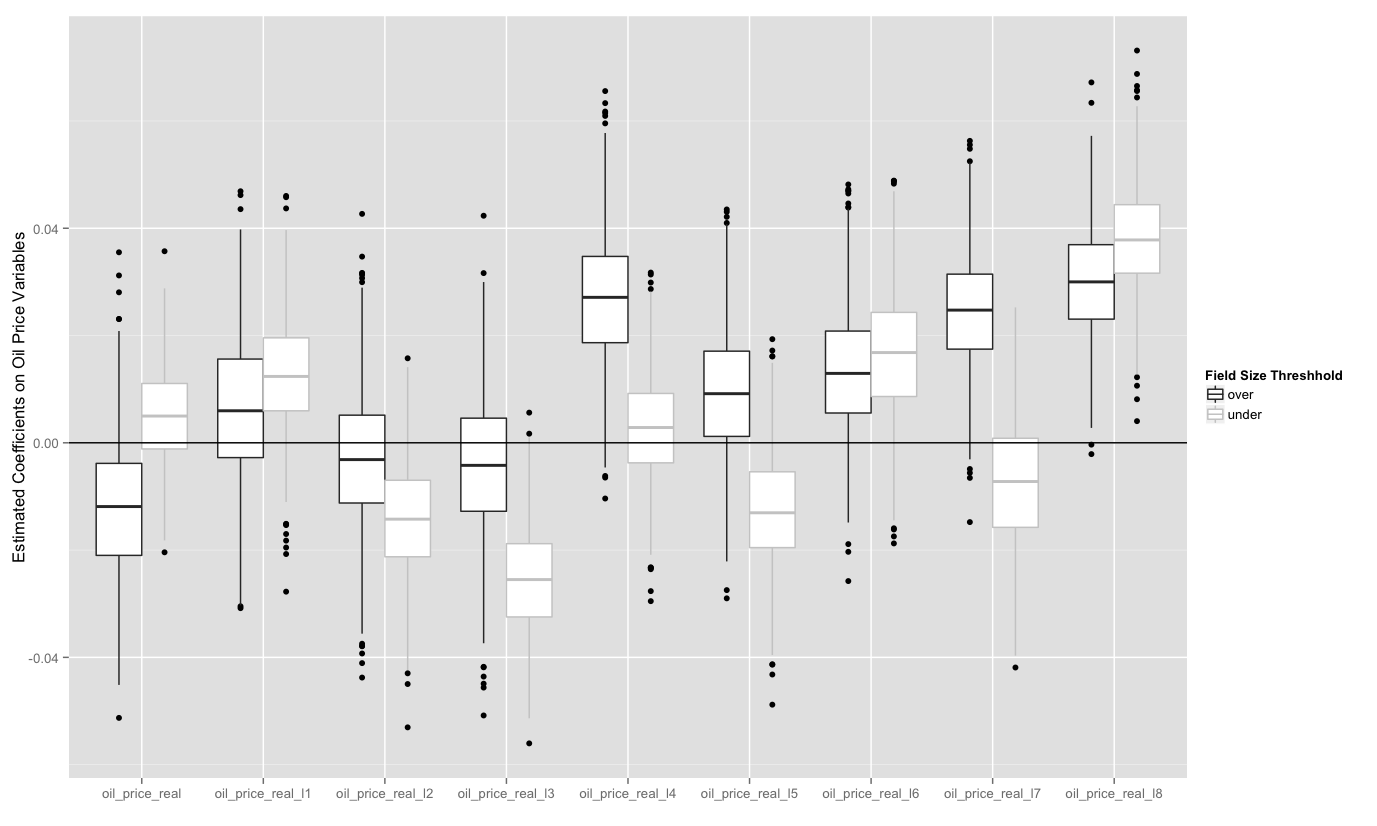
\includegraphics[width=1\textwidth]{figures/gam_price_8_print.png}
	\label{gam_price_8}
\end{figure}
\end{frame}

\begin{frame}
\begin{figure}
	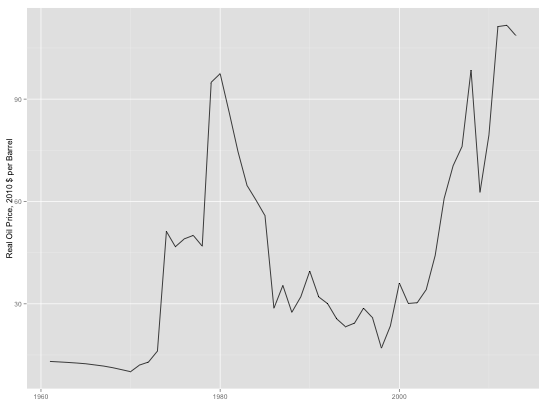
\includegraphics[width=1\textwidth]{figures/oil_price_series.png}
	\label{oil_price_series}	
\end{figure}
\end{frame}


\begin{frame}[plain, fragile]
	\begin{verbatim}
	fieldSize <- exp(rnorm(77, mean=2.3, sd=1.5))
	\end{verbatim}
\end{frame}


\begin{frame}[plain, fragile]
	\small \begin{verbatim}
	genyear<-function(size, maxsize){
		#let small fields be distributed uniformly from 1975 to 2013
		if(size<10){
			year<-trunc(runif(1, 1975, 2008))	
		} 
	\end{verbatim}
\end{frame}





\begin{frame}[plain, fragile]
	\small \begin{verbatim}
		else{
			range<-FALSE
			while(range==FALSE){
				year<-trunc(rnorm(1,mean=(1973+(maxsize+300)/(size+300)), sd=10))
				ifelse(year>=1970 & year<=2013, range<-TRUE, range<-FALSE)
				}	
			}
	return(year)
	}
	\end{verbatim}	
\end{frame}





\begin{frame}[plain]
	\begin{equation}
		cumProd=\frac{size}{1+exp(\frac{-prodTime_t}{3})}
		\label{cumProd_equation}
	\end{equation}
\end{frame}


\begin{frame}[plain]
	\begin{equation}
		log(production) = f`(time) + beta*log(price) + epsilon
	\end{equation}
\end{frame}

\begin{frame}[plain]
	\begin{figure}
		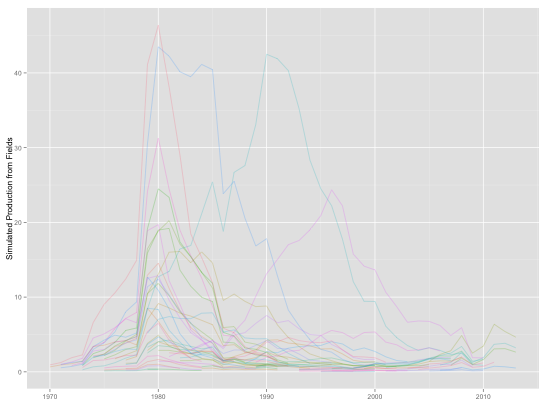
\includegraphics[width=1\textwidth]{figures/simulated_production.png}
		\caption{Simulated production of 77 oil fields}
		\label{simulated_production}	
	\end{figure}
\end{frame}


\small \begin{frame}[plain, fragile]
	\small \begin{verbatim}
	formula_0=formula(log(prod)~time_to_peak + time_to_peak_sq +
	 time_to_peak_cu + peak_to_end + peak_to_end_sq + 
	 peak_to_end_cu + size + price)
	\end{verbatim}
\end{frame}

\begin{frame}[plain, fragile]
	\small \begin{verbatim}
	gamm_mc_0<-replicate(1000, gam_mc(beta=0,
	 formula=formula_0, use_true_prices=TRUE))
	\end{verbatim}
\end{frame}

\begin{frame}[plain]
	\begin{figure}
		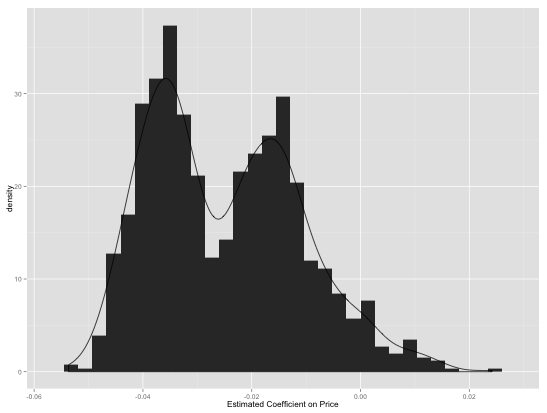
\includegraphics[width=1\textwidth]{figures/lin_model_price_mc.png}
		\caption{Estimated coefficients on price from linear model from Monte Carlo Experiment}
		\label{lin_model_price_mc}	
	\end{figure}
\end{frame}

\begin{frame}[plain, fragile]
	\begin{verbatim}
	formula_1= formula(prod~s(prod_time,size) + price)
	\end{verbatim}
\end{frame}


\begin{frame}[plain]
	\begin{figure}
		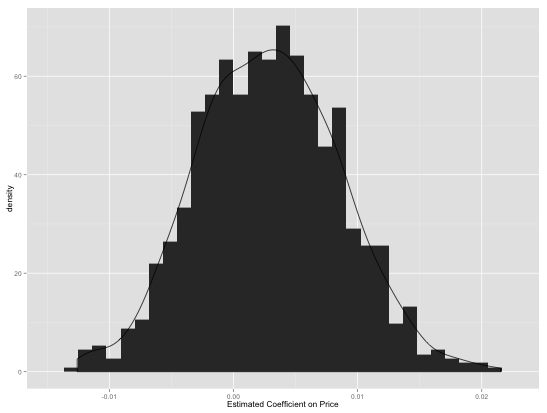
\includegraphics[width=1\textwidth]{figures/gam_model_price_mc.png}
		\caption{Estimated coefficients on price from GAM model from Monte Carlo Experiment}
		\label{gam_model_price_mc.png}	
	\end{figure}
\end{frame}



\begin{frame}[plain]
	Extensions
	\begin{itemize}
		\item Computation and estimation of efficiency, power of estimators
		\item Comparison of stationary and non stationary simulated price series
		\item Using monte carlo to generate uncertainty of oil production forecasts
	\end{itemize}
\end{frame}


\end{document}